\let\negmedspace\undefined
\let\negthickspace\undefined
\documentclass[journal]{IEEEtran}
\usepackage[a5paper, margin=10mm, onecolumn]{geometry}
%\usepackage{lmodern} % Ensure lmodern is loaded for pdflatex
\usepackage{tfrupee} % Include tfrupee package

\setlength{\headheight}{1cm} % Set the height of the header box
\setlength{\headsep}{0mm}     % Set the distance between the header box and the top of the text

\usepackage{gvv-book}
\usepackage{gvv}
\usepackage{cite}
\usepackage{amsmath,amssymb,amsfonts,amsthm}
\usepackage{algorithmic}
\usepackage{graphicx}
\usepackage{textcomp}
\usepackage{xcolor}
\usepackage{txfonts}
\usepackage{listings}
\usepackage{enumitem}
\usepackage{mathtools}
\usepackage{gensymb}
\usepackage{comment}
\usepackage[breaklinks=true]{hyperref}
\usepackage{tkz-euclide} 
\usepackage{listings}
% \usepackage{gvv}                                        
\def\inputGnumericTable{}                                 
\usepackage[latin1]{inputenc}                                
\usepackage{color}                                            
\usepackage{array}                                            
\usepackage{longtable}                                       
\usepackage{calc}                                             
\usepackage{multirow}                                         
\usepackage{hhline}                                           
\usepackage{ifthen}                                           
\usepackage{lscape}
\begin{document}

\bibliographystyle{IEEEtran}
\vspace{3cm}

\title{NCERT-8.1.ex.5}
\author{EE24BTECH11065 - Spoorthi yellamanchali
}
% \maketitle
% \newpage
% \bigskip
{\let\newpage\relax\maketitle}

\renewcommand{\thefigure}{\theenumi}
\renewcommand{\thetable}{\theenumi}
\setlength{\intextsep}{10pt} % Space between text and floats


\numberwithin{equation}{enumi}
\numberwithin{figure}{enumi}
\renewcommand{\thetable}{\theenumi}


\textbf{Question:}
\\
Find the area bounded by the ellipse $\frac{x^2}{a^2}$+$\frac{y^2}{b^2}$ = 1 and the ordinates $x=0$ and $x = ae$, where, $b^2 = a^2\brak{1 - e^2}$ and $e < 1$.
\\
\textbf{ Theoretical Solution: }
On substituting $x = ae$ and $b^2 = a^2\brak{1 - e^2}$,we get,
\begin{align}
    \frac{\brak{ae}^2}{a^2} + \frac{y^2}{a^2\brak{1 - e^2}} = 1
\end{align}
\begin{align}
     e^2 + \frac{y^2}{a^2\brak{1 - e^2}} = 1
\end{align}
\begin{align}
    \frac{y^2}{a^2\brak{1 - e^2}} = 1 - e^2
\end{align}
\begin{align}
    y^2 = a^2\brak{1 - e^2}^2
\end{align}
\begin{align}
     y = \abs{a\brak{1 - e^2}}
\end{align}
\begin{align}
    y = \pm  a\brak{1 - e^2}
\end{align}
From the equation of ellipse , we can write the expression for y as,
\begin{align}
    y = \pm \frac{b}{a}\sqrt{a^2 - x^2}
\end{align}
Area $A$ enclosed is equal to 
\begin{align}
    A = 2\int_0^{ae} \frac{b}{a}\sqrt{a^2 - x^2}\,dx
    \end{align}
    \begin{align}
      = \frac{2b}{a}\left[ae\sqrt{a^2 - \brak{ae}^2} + a^2\sin^{-1}{e} \right]
      \end{align}
\begin{align}
      = ab\left[e\sqrt{1 - e^2} + \sin^{-1}{e}\right]
\end{align}
\textbf{Solution by using the trapezoidal rule:}
\\
In the trapezoidal rule,we calculate the area of the curve by breaking the whole area into trapeziums of small areas and adding them up.\\
Under trapezoidal rule,Area $A$ is approximated by,
\begin{align}
    J = \int_a^b f(x)\,dx \approx h\brak{\frac{1}{2}\brak{f(a) + f(x_1)} + \frac{1}{2}\brak{f(x_1) + f(x_2)} + ..........+ \frac{1}{2}\brak{f(x_{n-1})+ f(b)}}
\end{align}
\begin{align}
    J = \int_a^b f(x)\,dx \approx h\brak{\frac{1}{2}f(a) + f(x_1) + f(x_2) + ..... + f(x_{n-1} + \frac{1}{2}f(b)}
\end{align}
Where $h$ is assumed to be the distance between parallel sides of trapezium and its value is taken close to zero.\\
so we the number of trapeziums the required area is broken into can be written as,
\begin{align}
    n = \frac{b - a}{h}
\end{align}
and,
On observing equation $\brak{0.11}$, we can see that,\\
If $A\brak{x_n}$ is area enclosed by the curve $f\brak{x}$, from $x=x_0$ to $x=x_n$,then,
\begin{align}
    A\brak{x_n} = A\brak{x_{n-1}} + \frac{1}{2}h\brak{f\brak{x_{n-1}} + f\brak{x_n}}
\end{align}
From the method of finite differences , we know that,
\begin{align}
    x_n = x_{n-1} + h
\end{align}
\begin{align}
    y_{n} = y_{n-1} + h\brak{\frac{dy}{dx}|_{x=x_{n-1}}}
\end{align}
On differentiating equation $\brak{as}$, and substituting the expression for $\frac{dy}{dx}$ in equation $\brak{a}$, we get the difference equation for the curve which is,
\begin{align}
     y_{n} = y_{n-1} + h\brak{\frac{-bx}{a\sqrt{a^2 - x^2}}}
\end{align}
\begin{align}
  A_{n+1}&=A_n+\frac{1}{2}h\brak{\brak{y_{n}+hy^{\prime}_n}+y_n}\\
  A_{n+1}&=A_n+\frac{1}{2}h\brak{2y_n+hy^{\prime}_n}\\
  A_{n+1}&=A_n+hy_n+\frac{1}{2}h^2y^{\prime}_n\\
\end{align}
In the given question, $y_n=\frac{b}{a}\sqrt{a^2-x_n^2}$ and $y^{\prime}_n= \frac{-bx_n}{\brak{a\sqrt{a^2-x_n^2}}}$\\
The general difference equation will be given by
\begin{align}
  A_{n+1}&=A_n+hy_n+\frac{1}{2}h^2y^{\prime}_n\\
  A_{n+1}&=A_n+h\brak{\frac{b}{a}\sqrt{a^2-x_n^2}}+\frac{1}{2}h^2\brak{\frac{-bx_n}{\brak{\sqrt{a^2-x_n^2}}}}\\
\end{align}
We know that,
\begin{align}
    x_0 = a\\
    x_n = ae
\end{align}
On changing different values of $h$, we will observe that,as value for $h$ approaches zero,the area calculated using trapezoidal rule approaches the area calculated theoretically.
On assuming a value fro $h$ close to zero and substituting in equation and on iterating till we reach $x_n=ae$ will return an area.\\
$\therefore$ our required area is twice the returned area.\\

For example,\\
let us take $a = 4$,$e = \frac{\sqrt{7}}{4}$ and observe for different $h$ values.
\begin{enumerate}
    \item  $h = 0.1$\\
    In this case we get, \\
Theoretical area is:  14.625751423656318\\
Area using trapezoidal rule:  14.870164029287624\\
\item $h = 0.01$\\
Theoretical area is:  14.625751423656318\\
Area using trapezoidal rule:  14.644880662091099\\
\item $h = 0.001$
Theoretical area is:  14.625751423656318\\
Area using trapezoidal rule:  14.626870703450807\\
\end{enumerate}

For our plot , Let , $a = 4$,$b = 3$,$h = 0.001$
\begin{figure}[h!]
   \centering
   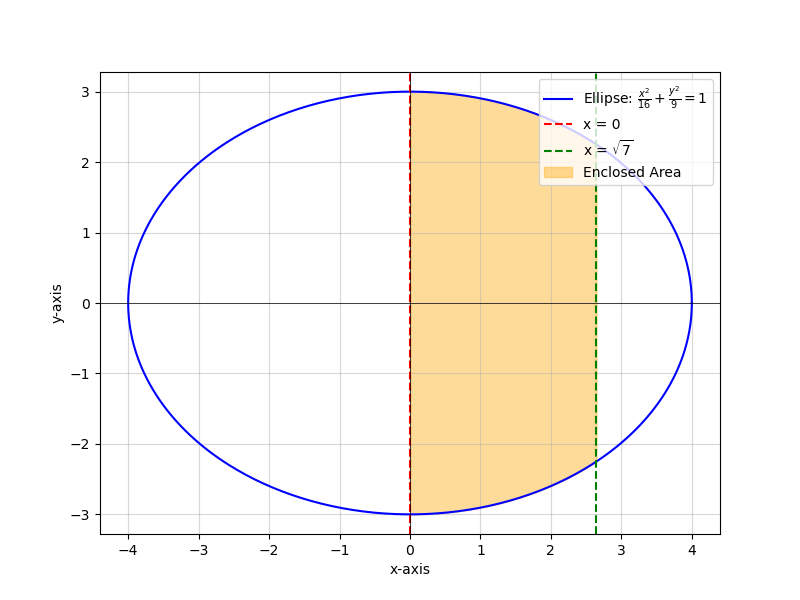
\includegraphics[width=0.75\columnwidth]{figures/Figure_1.png}
\end{figure}

\end{document}


